\documentclass[sigconf]{acmart}

\usepackage{comment, graphicx, algorithm, algorithmic, listings}


\lstdefinelanguage{P4}{
  showlines=true,
  morecomment=[f]{//},
  keepspaces=true,
  basicstyle=\scriptsize\ttfamily,
  emphstyle=\itshape,
  emph={},
  commentstyle=\color{red},
  keywordstyle=\color{blue},
  morekeywords={typedef, header, extern, struct, parser, state, transition, in, out, inout, select, default, control, action, table, apply, if, switch}
}



\AtBeginDocument{%
	\providecommand\BibTeX{{%
			\normalfont B\kern-0.5em{\scshape i\kern-0.25em b}\kern-0.8em\TeX}}}

%% Rights management information.  This information is sent to you
%% when you complete the rights form.  These commands have SAMPLE
%% values in them; it is your responsibility as an author to replace
%% the commands and values with those provided to you when you
%% complete the rights form.
\setcopyright{acmcopyright}
\copyrightyear{2018}
\acmYear{2018}
\acmDOI{10.1145/1122445.1122456}

%% These commands are for a PROCEEDINGS abstract or paper.
%%\acmConference[Woodstock '18]{Woodstock '18: ACM Symposium on Neural
%%  Gaze Detection}{June 03--05, 2018}{Woodstock, NY}
%%\acmBooktitle{Woodstock '18: ACM Symposium on Neural Gaze Detection,
%%  June 03--05, 2018, Woodstock, NY}
%%\acmPrice{15.00}
%%\acmISBN{978-1-4503-XXXX-X/18/06}

\begin{document}
	
	
	\title{TODO}
	
	
	\author{}
	\email{}
	\orcid{}
	\author{}
	\authornotemark[]
	\email{}
	\affiliation{%
		\institution{}
		\streetaddress{}
		\city{}
		\state{}
		\country{}
		\postcode{}
	}
	
	
	\begin{abstract}
		TODO
	\end{abstract}
	
	%%
	%% The code below is generated by the tool at http://dl.acm.org/ccs.cfm.
	%% Please copy and paste the code instead of the example below.
	%% TODO

	
	\keywords{TODO}
	
	
	\maketitle
	
	\section{Introduction}
	% P4 (max 1-1.5 hasáb) - példa (később használandó a többihez) - Máté
	
	\section{Related Work}
	% kb 1.5 hasáb
	% felhasznált eszközök  - 
	% egyéb toolok - Vera,  - Gabi
	% Akár gremlin/gráf alapú dolgok, ami nem p4 (akár refactorerl) - mindenki
	

	\section{Motivation}
	% max 1 hasáb - lehet intorba megy - Máté
	% p4-re vannak elemzések kéne fejlesztés segítő eszköz
	% ehhez egységes keretrendszer - vannak már ilyesmik related workben
	
	\section{Analysis framework}



	\subsection{Representation - Architecture} % 4 hasáb - Dániel
	% belső gráf, a koncepció
	% elemzések
	% app megvalósítás

  \begin{figure}
    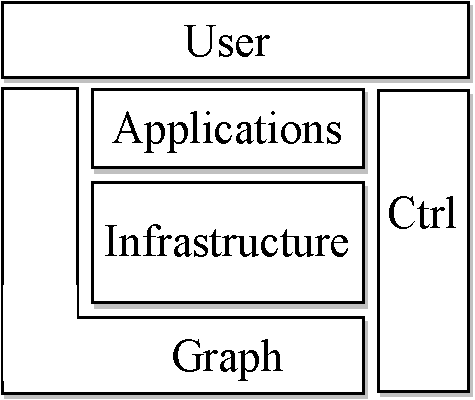
\includegraphics[width=0.18\textwidth]{figures/arch-top.pdf}
    \caption{TODO}\label{fig:arch-top}
  \end{figure}

  \begin{itemize}
    \item Figure \ref{fig:arch-top} 
    \item User extracts information (including metrics, object codes, verified properties) from the code using applications (corresp. backends). Applications provide services by utilizing the code knowledge stored in the knowledge graph by the analysers of the infrastructure layer (corresp. frontend). The collaboration of the application and the analysers is orchestrated by a controller module.
  \end{itemize}
	
	\subsection{Experts} % 1 hasáb - Dániel
	% kisebb gráf ábra

  \begin{figure}
    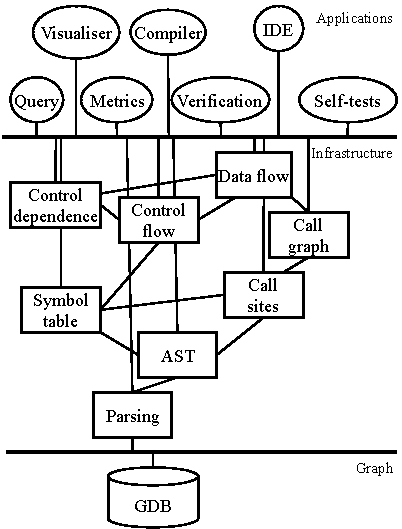
\includegraphics[width=0.3\textwidth]{figures/arch-deps.pdf}
    \caption{TODO}\label{fig:arch-deps}
  \end{figure}

  \begin{itemize}
    \item Figure \ref{fig:arch-deps} 
    \item More granular.
    \item Analysers depend on each other. Applications only depend on one or more analysers.
    \item Controller manages dependencies.
  \end{itemize}
	

	\subsection{Testing} % 1 hasáb - Gabi
	% külön modul
	% elvi részei jelenlenek meg
	% ilyen olyan teszt, messziről melyik hogy
	
	\section{Evaluation}
	
	% scalability measurements  talán 1 hasáb
	% esetleg 1-2 plre hogy futott le - sor alapján? mini mérés
	
	% indítási információk - mindegyiknél /visualisation-nél
	% egyedi elemzések mérése
	\subsection{Visualization} % 0.5 hasáb
	\subsection{Verification} % 1 hasáb - Gabi
	\subsection{Cost analysis} % 1 hasáb - Dániel
	
	\section{Conclusion and Future Work} % 1 hasáb - Máté

\begin{figure*}
\begin{tabular}{|p{3.3cm}|p{5.9cm}|p{7.7cm}|}
\hline
\begin{lstlisting}[language=P4]
// Definitions
typedef bit<9>  egSpec_t;
typedef bit<48> macAddr_t;
typedef bit<32> ip4Addr_t;

// Headers
header ethernet_t {
  macAddr_t dstAddr;
  macAddr_t srcAddr;
  bit<16>   etherType; }
    
header ipv4_t {
  bit<8>    ttl;
  ip4Addr_t srcAddr;
  ip4Addr_t dstAddr;... }
    
struct headers {
  ethernet_t   ethernet;
  ipv4_t       ipv4; }

\end{lstlisting}
&
\begin{lstlisting}[language=P4]
// Parser
parser MyParser(...) {
  state start { transition parse_ethernet; }
  state parse_ethernet {
    packet.extract(hdr.ethernet);
    transition select(hdr.ethernet.etherType) {
      TYPE_IPV4: parse_ipv4;
      default: accept; } }
  state parse_ipv4 {
    packet.extract(hdr.ipv4);
    transition accept; } }
    
// Control    
control MyIngress(...) {
  apply {
    if (hdr.ipv4.isValid()) {
           ipv4_lpm.apply(); }
  }         
  action drop() {
    mark_to_drop(standard_metadata);
  }    
\end{lstlisting}
&
\begin{lstlisting}[language=P4]
  action ipv4_forward(macAddr_t dstAddr, egSpec_t port) {
    standard_metadata.egress_spec = port;
    hdr.ethernet.srcAddr = hdr.ethernet.dstAddr;
    hdr.ethernet.dstAddr = dstAddr;
    hdr.ipv4.ttl = hdr.ipv4.ttl - 1;
  }    
  table ipv4_lpm {
    key = {  hdr.ipv4.dstAddr: lpm;  }
    actions = {
      ipv4_forward;
      drop;
      NoAction;}
    ... }   
}

//Deparser
control MyDeparser(packet_out packet, in headers hdr) {
  apply {
    packet.emit(hdr.ethernet);
    packet.emit(hdr.ipv4);}
}
\end{lstlisting}\\
\hline
\end{tabular}
\caption{P4 example}
  \label{code:P4}
\end{figure*}

	
\end{document}
\endinput

